\documentclass[a4paper,12pt]{article}

\usepackage[utf8]{inputenc}
\usepackage[T1]{polski}
\usepackage{helvet}
\usepackage{graphicx}
\usepackage{color}
\usepackage{geometry}
\usepackage[style=numeric,backend=bibtex,sorting=none]{biblatex}
\usepackage{indentfirst}
\usepackage[labelfont=bf]{caption}
\usepackage{setspace}
\usepackage{placeins}
\usepackage{xcolor}
\usepackage{listings}
\usepackage{accsupp}

\newcommand*{\noaccsupp}[1]{\BeginAccSupp{ActualText={}}#1\EndAccSupp{}}

\newcommand{\comment}[1]{}

\lstdefinestyle{shared}{
    numbers=left,
    numbersep=1em,
    numberstyle=\tiny\color{black}\noaccsupp,
    frame=single,
    framesep=\fboxsep,
    framerule=\fboxrule,
    rulecolor=\color{black},
    xleftmargin=\dimexpr\fboxsep+\fboxrule\relax,
    xrightmargin=\dimexpr\fboxsep+\fboxrule\relax,
    breaklines=true,
    tabsize=2,
    columns=flexible,
    captionpos=t,
    escapeinside={(*@}{@*)},
}

\lstdefinestyle{python}{
    style=shared,
    language={Python},
    basicstyle=\linespread{1}\small\tt,
    keywordstyle=\color{blue},
    commentstyle=\color[rgb]{0.13,0.54,0.13},
    morekeywords={
        Console,
        WriteLine,
        int,
    },
}

\lstdefinestyle{cpp}{
    style=shared,
    language={C++},
    basicstyle=\linespread{1}\small\tt,
    keywordstyle=\color{blue},
    commentstyle=\color[rgb]{0.13,0.54,0.13},
    morekeywords={},
}

\lstnewenvironment{python}[1][]{
    \lstset{style=python,#1}
}{}

\lstnewenvironment{cpp}[1][]{
    \lstset{style=cpp,#1}
}{}

\addbibresource{bibliography.bib}
\DefineBibliographyStrings{english}{
  january = {Styczeń},
  february = {Luty},
  march = {Marzec},
  april = {Kwiecień},
  may = {Maj},
  june = {Czerwiec},
  july = {Lipiec},
  august = {Sierpień},
  september = {Wrzesień},
  october = {Październik},
  november = {Listopad},
  december = {Grudzień},
}

\newenvironment{dedication}{
  \clearpage
  \vspace*{\stretch{4}}
  \itshape
  \raggedleft
  }{
  \par
  \vspace{\stretch{1}}
  \clearpage
}

\geometry{hmargin={2cm, 2cm}, height=10.0in}

\begin{document}

% !TEX root = main.tex
\thispagestyle{empty}
%% ------------------------ NAGLOWEK STRONY ---------------------------------

\includegraphics[height=37.5mm]{img/agh_nzw_a_pl_1w_wbr_cmyk}\\
\rule{30mm}{0pt}
{\large \textsf{Wydział Fizyki i Informatyki Stosowanej}}\\
\rule{\textwidth}{3pt}\\
\rule[2ex]
{\textwidth}{1pt}\\
\vspace{7ex}
\begin{center}
{\LARGE \bf \textsf{Praca magisterska}}\\
\vspace{13ex}
% --------------------------- IMIE I NAZWISKO -------------------------------
{\bf \Large \textsf{Piotr Sarna}}\\
\vspace{3ex}
{\sf\small kierunek studiów:} {\bf\small \textsf{informatyka stosowana}}\\
\vspace{1.5ex}
{\sf\small specjalność:} {\bf\small \textsf{modelowanie i analiza danych}}\\
\vspace{10ex}
%% ------------------------ TYTUL PRACY --------------------------------------
{\bf \huge \textsf{Równoległe przetwarzanie przypadków w systemie wyzwalania eksperymentu ATLAS}}\\
\vspace{14ex}
%% ------------------------ OPIEKUN PRACY ------------------------------------
{\Large Opiekun: \bf \textsf{dr hab. inż. Tomasz Bołd}}\\
\vspace{22ex}
{\large \bf \textsf{Kraków, sierpień 2019}}
\end{center}
%% =====  STRONA TYTUŁOWA PRACY MAGISTERSKIEJKIEJ ====

\newpage

%% =====  TYŁ STRONY TYTUŁOWEJ PRACY MAGISTERSKIEJKIEJ ====
{\sf Oświadczam, świadomy(-a) odpowiedzialności karnej za poświadczenie nieprawdy, że niniejszą pracę dyplomową wykonałem(-am) osobiście i samodzielnie i  nie korzystałem(-am) ze źródeł innych niż wymienione w pracy.}

\vspace{14ex}

\begin{center}
\begin{tabular}{lr}
~~~~~~~~~~~~~~~~~~~~~~~~~~~~~~~~~~~~~~~~~~~~~~~~~~~~~~~~~~~~~~~~~ &
................................................................. \\
~ & {\sf (czytelny podpis)}\\
\end{tabular}
\end{center}

%% =====  TYL STRONY TYTULOWEJ PRACY MAGISTERSKIEJKIEJ ====

\newpage
\rightline{Kraków, ?? czerwca 20??}
\begin{center}
{\bf Tematyka pracy magisterskiej i praktyki dyplomowej
Jana Nowaka,
studenta V roku studiów kierunku fizyka techniczna, specjalności fizyka komputerowa}\\
\end{center}

Temat pracy magisterskiej:
{\bf Równoległe przetwarzanie przypadków w systemie wyzwalania eksperymentu ATLAS}\\

\begin{tabular}{rl}

Opiekun pracy:                  & dr hab. inż. Tomasz Bołd\\
Recenzenci pracy:               & //TODO\\
Miejsce praktyki dyplomowej:    & WFiIS AGH, Kraków\\
\end{tabular}

\begin{center}
{\bf Program pracy magisterskiej i praktyki dyplomowej}
\end{center}

\begin{enumerate}
\item Omówienie realizacji pracy magisterskiej z opiekunem.
\item Zebranie i opracowanie literatury dotyczącej tematu pracy.
\item Praktyka dyplomowa:
\begin{itemize}
\item zapoznanie się z ideą...,
\item uczestnictwo w eksperymentach/przygotwanie oprogramowania...,
\item dyskusja i analiza wyników...
\item sporządzenie sprawozdania z praktyki.
\end{itemize}
\item Kontynuacja obliczeń związanych z tematem pracy magisterskiej.
\item Zebranie i opracowanie wyników obliczeń.
\item Analiza wyników obliczeń numerycznych, ich omówienie i zatwierdzenie przez opiekuna.
\item Opracowanie redakcyjne pracy.
\end{enumerate}


\noindent
Termin oddania w dziekanacie: ?? czerwca 20??\\[1cm]

\begin{center}
\begin{tabular}{lcr}
.............................................................. & ~~~ &
.............................................................. \\
(podpis kierownika katedry) & & (podpis opiekuna) \\
\end{tabular}
\end{center}

\newpage

\noindent
Na kolejnych dwóch stronach proszę dołączyć kolejno recenzje pracy popełnione przez Opiekuna oraz Recenzenta (wydrukowane z systemu MISIO i podpisane przez odpowiednio Opiekuna i Recenzenta pracy). Papierową wersję pracy (zawierającą podpisane recenzje) proszę złożyć w dziekanacie celem rejestracji co najmniej na tydzień przed planowaną obroną.

\linespread{1.3}
\selectfont


% !TEX root = main.tex
\newpage
\tableofcontents
% !TEX root = main.tex
\begin{dedication}
Wszystkim,\break
którzy zawsze mieli dla mnie otwarte drzwi.
\end{dedication}

\section{Wstęp}
Celem niniejszej pracy jest opisanie narzędzia \mbox{GenericMonitoringTool} stworzonego w ramach modułu \mbox{AthenaMonitoring} stanowiącego część środowiska Athena i opisanie jak umożliwiło ono monitorowanie jakości danych w wielowątkowych algorytmach. 
Monitorowanie danych odbywa się poprzez generację histogramów i porównanie ich z referencjami. Opisane w pracy narzędzie dotyczy pierwszego kroku w tym procesie.
Histogramy używane są z tego powodu że pozwalają na kompaktowe podsumowanie istotnych cech dużego zbioru danych. 
W zastosowaniu do monitorowania jakości danych pozwalają na szybkie uchwycenie anomalii co w konsekwencji prowadzi do wdrożenia poprawek i polepszenia jakości danych czy wręcz do zlokalizowania krytycznych błędów w konfiguracji eksperymentu. 

\subsection{Eksperyment ATLAS}
ATLAS~\cite{cern-atlas} jest jednym z czterech głównych eksperymentów w ramach Wielkiego Zderzacza Hadronów(LHC)~\cite{cern-lhc} w ośrodku naukowym CERN. 
Jest to eksperyment fizyki cząstek elementarnych ogólnego przeznaczenia prowadzony przez międzynarodową grupę naukowców. 
Został zaprojektowany w celu pełnego wykorzystania potencjału odkrywczego i ogromnego zakresu możliwości fizycznych, jakie zapewnia LHC.

\subsection{Athena}
Athena~\cite{cern-athena} jest platformą programistyczną, która umożliwia pracę z danymi pochodzącymi z eksperymentu ATLAS. 
Obejmuje to m.in. filtracji danych, generowanie przypadków zdarzeń metodami Monte-Carlo, symulacje odpowiedzi detektora oraz rekonstrukcję danych. 
Jego głównymi komponentami są algorytmy, które analizują i przekształcają dane pochodzące z eksperymentu. 
Pozostałe komponenty środowiska to narzędzia (tools), za pomocą których implementowany jest wzorzec strategia. 
Komponenty te pisane są w języku C++ a konfigurowane z użyciem skryptów napisanych w języku Python. 

\subsection{ROOT}
ROOT~\cite{cern-root} jest środowiskiem stworzonym w CERN i Fermilab, które umożliwia pracę z wielkimi zbiorami danych, w celu ich statycznej analizy, wizualizacji i przechowywania. 
Został on stworzony w języku C++ przez co dobrze komponuje się z frameworkiem Athena i jest w nim używany na potrzeby prezentowania wyników działania algorytmów. 

\subsection{AthenaMonitoring i GenericMonitoringTool}
AthenaMonitoring~\cite{atlas-athena-monitoring} jest modułem stworzonym w ramach frameworka Athena.
Dostarcza on niezbędne narzędzia do monitorowania przebiegu algorytmów i tworzenia na ich podstawie histogramów ROOT.
Proces monitoringu jest ważny dlatego, że ilość danych produkowanych przez Eksperyment ATLAS jest ogromna i jedynym sposobem, aby móc je przeanalizować są wykresy i histogramy.
Pozwalają one znaleźć odchyły od normy w danych pochodzących z eksperymentu, oraz ułatwiają obserwacje zależności pomiędzy różnymi zbiorami danych.
Podwyższa to jakość pozyskanych danych i ułatwia rozwiązywanie ewentualnych problemów.

W ramach tego modułu stworzone zostało narzędzie GenericMonitoringTool. 
Jego głównym zadaniem jest umożliwienie, w przystępny dla użytkownika sposób, dodania funkcjonalności monitoringu do algorytmów.
Realizuje to poprzez dostarczenie zbioru klas użytecznych w procesie adaptacji kodu. 
Zostało ono zaprojektowane z myślą o jak największej transparentności użycia, przy jednoczesnym zapewnieniu elastyczności konfiguracji i bezpieczeństwa przy wykorzystaniu wielowątkowym.
% !TEX root = main.tex
\section{Refaktoryzacja}
\comment{https://pl.wikipedia.org/wiki/Refaktoryzacja}
\comment{Czysty Kod - Robert C. Martin}
Refaktoryzacja (ang. refactoring) jest to proces zwiększania jakości istniejącego kodu źródłowego, bez modyfikacji jego funkcjonalności. Jest to niezbędna część zarządzania projektem informatycznym, która pozwala utrzymać czytelny i dobrze zorganizowany kod, dostosowany do szeroko znanych wzorców projektowych. Dzięki stosowaniu takich praktyk, okres wdrażania nowych osób do projektu jest krótszy, zmniejsza się narzut na utrzymanie kodu oraz dodawanie nowych funkcjonalności - szczególnie zmian afektujących wiele komponentów jednocześnie. 

Działania, które wykonuje się w ramach refaktoryzacji to:
\begin{itemize}
\item zmiana nazw zmiennych, funkcji i klas na bardziej opisowe
\item ograniczenie liczby parametrów przekazywanych do funkcji
\item ograniczenie długości definicji funkcji
\item dostosowanie elementów systemu do przyjętych w projekcie standardów i wzorców
\item wydzielenie podobnych funkcjonalności w celu usunięcia zduplikowanego kodu
\item określenie odpowiedzialności poszczególnych komponentów celem identyfikacji zbyt skomplikowanych struktur
\item przygotowanie kodu do testowania (np. umożliwienie wstrzykiwania zależności) i napisanie testów
\end{itemize}

Refaktoryzacja jako proces jest kosztowna, gdyż nie zostaje wytworzona żadna nowa funkcjonalność, oraz z perspektywy użytkownika zachowanie programu nie ulega zmianie. Lecz jest ona wartością samą w sobie, która rekompensuje koszt wprowadzania późniejszych zmian w projekcie - szczególnie w dużych i długożyjących projektach.


\comment{https://mfiles.pl/pl/index.php/Refactoring}
Jeśli istniejący kod jest zły na tyle, że pomimo możliwości zastosowania procesu refaktoryzacji, najprościej będzie napisać go od nowa. Taka sytuacja powinna mieć miejsce, kiedy program nie działa. Błędy mogą być odkryte podczas procesu testowania. Przed zastosowaniem refaktoryzacji program powinien działać bez komplikacji.

\comment{
\begin{itemize}
\item opisać proces, jak przebiegała
\item zebranie wymagań dot. refaktorowanego kodu
\item czemu czasem łatwiej przepisać
\item utworzenie interfejsu przyjaznego użytkownikowi
\item architektura nowego rozwiązania
\end{itemize}
}
% !TEX root = main.tex
\section{Obecna implementacja modułu AthenaMonitoring}
Dotychczas środowisko Athena używało jednowątkowego przetwarzania algorytmów. 
Ich sekwencja wykonania jest z góry określona przez pliki konfiguracyjne napisane w Pythonie. 
Służą one również do wystartowania całego zadania, np. rekonstrukcji. 
Algorytmy współdzielą dane poprzez pisanie i odczytywanie ich ze wspólnego magazynu danych (Event Store). 
Mogą one również używać narzędzi, które są konfigurowane niezależnie. 
Algorytmy mogą wchodzić w interakcję z serwisami, których cykl życia jest niezależny od cyklu wykonania algorytmów.
W kontekście monitoringu, najważniejszy jest serwis do histogramowania (THistSvc), który zajmuje się zapisywaniem histogramów ROOT na dysk. 
Schemat wykonania rekonstrukcji został pokazany na \figref{fig:athena:oldFlow}.

\begin{figure}[!ht]
\centering
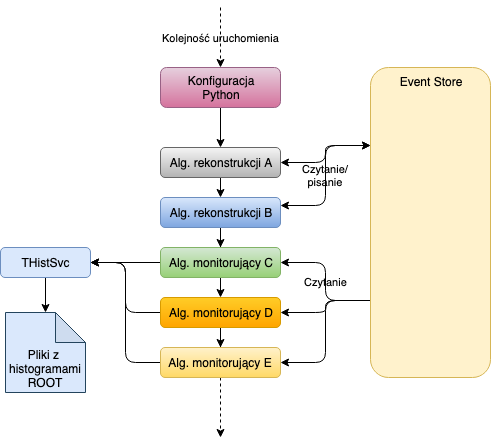
\includegraphics[width=0.75\textwidth]{img/old_flow.png}
\caption{
Schemat prezentuje proces wykonania kodu w aktualnej implementacji środowiska Athena. 
Kolejność algorytmów jest sztywno zdefiniowana w pliku konfiguracyjnym, w którym algorytmy monitorujące wykonywane są po algorytmach rekonstrukcji, które te dane produkują. 
Następnie algorytmy monitorujące komunikują się z serwisem THistSvc w celu zapisania gotowych histogramów do plików ROOT.
}
\label{fig:athena:oldFlow}
\end{figure}

Taka implementacja modułu do monitorowania i algorytmów niesie za sobą następujące niepożądane konsekwencje:

\begin{itemize}
\item twórca algorytmu ma bezpośredni i nieograniczony dostęp do wskaźników na histogramy ROOT. 
W związku z tym, niemożliwe jest zarządzanie takim kodem z centralnego miejsca.
Jego użytkownik, w każdej chwili, może wpłynąć na jego zachowanie i zmienić parametry wykonania.
Co więcej, adaptacja do nowych wersji ROOTa jest całkowicie zależna od autora algorytmu. Powoduje to, że framework musi zawsze zachowywać kompatybilność wsteczną, żeby kod Athena nie przestał działać.
\comment{Z tego powodu klasy ROOT rozrastają się do kilku tysięcy linii. }
\item deklaracja parametrów histogramów dzieje się w kodzie C++ napisanym przez użytkownika. 
W związku z tym drobne zmiany i poprawki binowania histogramów, wymagają nowego wersji frameworka Athena. 
Jest to szczególnie uciążliwe, gdy warunki uruchomienia dynamicznie się zmieniają, a nieprawidłowe binowanie prowadzi np. do umieszczenia w większości wyników poza zakresem.
\item najczęściej używanymi klasami z frameworka ROOT są TH1, TGraph, TTree. 
Ich interfejs jest do siebie bardzo zbliżony. 
Jednakże każdy z tych typów wymaga specjalnego kodu do ich poprawnej obsługi. 
Więc jeśli programista nie będzie postępował dokładnie z wytycznymi z dokumentacji, może to prowadzić do trudnych do wykrycia błędów. 
\end{itemize}

\subsection{Problem mergeowania}

\comment{
\begin{itemize}
\item co istniało do tej pory?
\item czemu potrzeba czegoś nowego?
\item wady starego rozwiązania
\item czemu monitoring jest ważny?
\item do czego jest używany?
\item na co pozwalał dotychczas?
\item WYDAJNOŚĆ
\item BEZPIECZEŃSTWO dla wielowątkowości
\item kto używa kodu, dostosowanie do klienta
\item co to Athena, gdzie jest uzywana, do czego, co to CERN, ile danych przetwarza
\item czemu nowe rozwiązanie pomoże unikać pomyłek w danych wejściowych!!!
\item co to algorytmy i filtrowanie ONLINe i OFFLINE
\item data quality
\end{itemize}
}
% !TEX root = main.tex
\section{Nowa implementacja modułu AthenaMonitoring}
Głównym celem refaktoringu framworka, było oddzielenie kodu odpowiedzialnego za zarządzanie histogramami od kodu algorytmów. 
Dzięki takiemu rozgraniczeniu odpowiedzialności, twórcy algorytmów mogą skupić się na ich poprawnej implementacji i określeniu które wartości powinny znaleźć się na wykresach jako wynik. 
Natomiast to kiedy stworzyć histogram, jak go wypełnić i zapisać jest obsługiwane przez wspólny kod. 

Sercem nowego rozwiązania jest GenericMonitoringTool - nowe narzędzie w ramach frameworka Athena.
Zajmuje się on przygotowaniem histogramów i powiązaniem ich z kodem uruchamianych algorytmów. 
Działa on w oparciu o deklaracje.
Twórca algorytmu deklaruje zbiór wartości (obejmuje to skalary oraz tablice) jakie mogą być monitorowane w obrębie jego wykonania, oraz informuje GenericMonitoringTool kiedy są one gotowe do przekazania do histogramów.
Natomiast użytkownik takiego algorytmu, deklaruje jakie wykresy chciałby stworzyć i z użyciem których zmiennych. 
Następuje to w kroku konfiguracyjnym Athena Python, gdzie definiuje on typy histogramów, parametry binowania, zakresy wartości, opisy itd. 
Taki interfejs pozwala uniknąć rekompilacji kodu C++ za każdym razem, gdy użytkownik zmienia parametry wykresu. 

\begin{figure}[!ht]
\centering
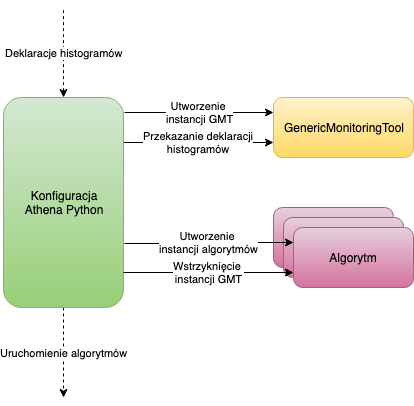
\includegraphics[width=0.75\textwidth]{img/algo_init.png}
\caption{
Przygotowanie instancji GenericMonitoringTool i monitorowanych algorytmów w konfiguracji Athena Python. Na tym etapie niezbędne jest zadeklarowanie histogramów, które powinny zostać utworzone jako wynik uruchomienia skryptu.
}
\label{fig:athena:oldFlow}
\end{figure}

\begin{figure}[!ht]
\centering
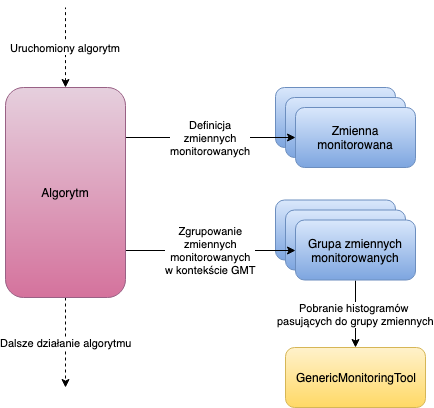
\includegraphics[width=0.75\textwidth]{img/algo_run.png}
\caption{
Przygotowanie zmiennych i grup w monitorowanym algorytmie, oraz przekazanie kontekstu do grupy w postaci instancji GenericMonitoringTool. Pozwala to skojarzyć zadeklarowane histogramy ze zmiennymi występującymi w tej grupie. 
}
\label{fig:athena:oldFlow}
\end{figure}

\subsection{Deklaracja histogramu}
Histogramy, które GenericMonitoringTool stworzy w ramach uruchomienia skryptu, muszą zostać wpierw zadeklarowane przez użytkownika w skrypcie Athena Python. Aby to zrobić należy przygotować łańcuch znaków w następującym formacie: 

\begin{center}
\begin{tabular}{l}
PATH, HTYPE, WEIGHT, CONV, VNAMES, TITLE, BINNING, [BLABELS], OPT
\end{tabular}
\end{center}

\begin{itemize}
\item PATH - ścieżka pod jaką zostanie utworzony histogram. Dostępne ścieżki najwyższego poziomu: EXPERT, SHIFT, DEBUG, RUNSTAT, EXPRESS
\item HTYPE - rodzaj histogramu. Musi być jednym z: TH1[F,D,I], TH2[F,D,I], TProfile, TProfile2D, TEfficiency
\item WEIGHT - nazwa zmiennej zawierającej wagi dla histogramu
\item CONV - konwencja dla ścieżek pod jaką zostanie utworzony histogram
\item VNAMES - nazwy zmiennych monitorowanych, które zostaną użyte do wypełnienia histogramu. Mogą być w formacie np. "name1,name2;alias", wtedy name1 i name2 będą nazwami zmiennych; natomiast name1 i alias, będą podpisami osi na histogramie
\item TITLE - tytuł histogramu
\item BINNING - zakresy wartości kolejnych osi histogramu. Ilość wartości w tym polu jest zależna od rodzaju histogramu
\item BLABELS - opcjonalne podpisy dla poszczególnych binów histogramu
\item OPT - dodatkowe opcje histogramu. Dostępne opcje: kCanRebin, Sumw2, kAddBinsDynamically, kLBNHistoryDepth=value, kCumulative, kVec, kVecUO
\end{itemize}

\subsection{Publiczny interfejs}

\subsubsection{GenericMonitoringTool}
Centralnym punktem nowej implementacji jest klasa GenericMonitoringTool, będąca narzędziem frameworka Athena.
Służy ona jako pomost pomiędzy konfiguracją napisaną w Pythonie, a kodem algorytmów w C++.
Jest zarządzana przez użytkownika i to do niej wstrzykuje się deklaracje histogramów jakie mają zostać utworzone podczas uruchomienia.
To ona odpowiada za przygotowanie i przechowywanie obiektów ROOT, wygenerowanych na podstawie tych deklaracji.
Dostęp do nich zapewnia poprzez warstwę abstrakcji zdefiniowaną w klasie HistogramFiller. 
Dodatkowo, posiada ona dostęp do aktualnych wartości Run Number i Lumi Block; dzięki temu możliwe jest generowanie grup histogramów w kontekście tych zmiennych. 
 
\subsubsection{HistogramDef}
Deklaracje histogramów na potrzeby GenericMonitoringTool reprezentowane są przez klasę HistogramDef.
To w niej zachodzi parsowanie ciągu znaków podanego przez użytkownika i wstępna weryfikacja jego poprawności.
Dzięki niej łatwiejszy jest dostęp do wybranych danych o histogramie. 
Jeśli parsowanie z jakiegoś powodu się nie powiedzie, użytkownik zostanie o tym poinformowany poprzez wyjątek, wraz z opisem problemu.

\subsubsection{IHistogramProvider}
Interfejs IHistogramProvider został przygotowany z myślą o zapewnieniu warstwy abstrakcji pomiędzy frameworkiem ROOT, a kodem do monitorowania zmiennych. 
Zawiera on jedną metodę - `histogram()`; to ona wykorzystywana jest, aby pobrać odpowiedni obiekt histogramu do wypełnienia.

\subsubsection{IMonitoredVariable}
Interfejs IMonitoredVariable stanowi bazę dla wszystkich zmiennych monitorowanych. 
Zawiera on nazwę zmiennej oraz metodę `getVectorRepresentation()`, która musi zostać zaimplementowana przez klasy pochodne.
Framework dostarcza gotowe implementacje tego interfejsu, jednak w specyficznych przypadkach użytkownik może sam go zaimplementować.  

\subsubsection{MonitoredScalar}
MonitoredScalar jest implementacją interfejsu IMonitoredVariable, reprezentującą pojedynczą wartość. 
Może ona być dowolnego typu, dopóki możliwe jest zrzutowanie go do `double`.
Definicja tej klasy pozwala wielokrotnie pobierać i modyfikować jej aktualną wartość.
Użytkownik może zdefiniować transformację tej zmiennej, która zostanie zaaplikowana w momencie pobrania jej wartości na potrzeby wypełnienia histogramu.

\subsubsection{MonitoredCollection}
MonitoredCollection jest implementacją interfejsu IMonitoredVariable, reprezentującą kolekcję wartości. 
Może ona być dowolnego typu, dopóki możliwe jest zrzutowanie wartości tej kolekcji do `double`.
Po utworzeniu obiektu tego typu, nie można go bezpośrednio modyfikować.
Jednak wszystkie zmiany przeprowadzone na kolekcji, zostaną odzwierciedlone w końcowym wyniku.
Użytkownik może zdefiniować transformację dla obiektów znajdujących się w kolekcji, która zostanie zaaplikowana w momencie pobrania ich wartości na potrzeby wypełnienia histogramu.

\subsubsection{MonitoredTimer}
MonitoredTimer jest implementacją interfejsu IMonitoredVariable, która pozwala mierzyć czas w mikrosekundach.
Dostarcza metody `start()` i `stop()`, zapewniające kontrole nad jej zachowaniem.
Wymagane jest, aby nazwy zmiennych tego typu posiadały prefix `TIME\_`.

\subsubsection{MonitoredGroup}
Miejscem w którym zmienne monitorowane kojarzone są z odpowiednimi histogramami jest klasa MonitoredGroup. 
Przyjmuje ona referencje do GenericMonitoringTool i zbioru IMonitoredVariable.
Na tej podstawie pobiera listę obiektów HistogramFiller, które są zapamiętywane w jej kontekście.
Dzięki temu możliwe jest określenie, kiedy i które histogramy należy wypełnić oraz jakie zmienne mają być użyte w tym celu.
Domyślnie wypełnienie następuje, gdy wywoływany jest destruktor obiektu MonitoredGroup. 
Jednakże, można to zrobić manualnie używając metody `fill()`.
Stworzenie obiektu MonitoredGroup jest niezbędne do używania zmiennych monitorowanych, ponieważ bez grupy, niemożliwe jest skojarzenie zmiennych z histogramami. 

\subsubsection{HistogramFiller}
Klasa abstrakcyjna HistogramFiller agreguje wszystkie dane niezbędne do poprawnego wypełnienia histogramów danymi. 
To ona przechowuje referencje do instancji IHistogramProvider, HistogramDef, zbioru IMonitoredVariable i mutexów.
Zapewnia interfejs do wypełniania histogramów w postaci metody `fill()`.
Klasy pochodne, powinny ją zaimplementować i wpisać dane ze zmiennych monitorowanych do histogramów ROOT.
W tej metodzie używany jest również mutex do zapewnienia spójności danych i synchronizacji pomiędzy różnymi wątkami. 

\subsubsection{HistogramDefParseException}
HistogramDefParseException reprezentuje błędy powstałe przy próbie sparsowania deklaracji histogramu dostarczonej przez użytkownika.
Zawiera on informacje o przyczynie problemu.

\subsubsection{HistogramException}
HistogramException reprezentuje błędy powstałe przy próbie utworzenia obiektów ROOT na podstawie HistogramDef.
Zawiera on informacje o przyczynie problemu.

\subsection{Niepubliczny interfejs}

\subsubsection{HistogramFactory}
Klasa HistogramFactory stanowi bezpośrednią warstwę komunikacji z serwisem THistSvc w którym tworzone są obiekty ROOT.
Odpowiada ona za interpretację HistogramDef, stworzenie histogramu odpowiedniego typu i skonfigurowanie go na podstawie tej deklaracji.
Dodatkowo zapewnia mechanizm ponownego użycia raz już stworzonych histogramów, co zwiększa wydajność tego rozwiązania.

\subsubsection{HistogramFillerFactory}
Głównym zadaniem klasy HistogramFillerFactory jest utworzenie odpowiedniego zestawu obiektów IHistogramProvider i HistogramFiller na podstawie dostarczonej definicji histogramu w kontekście GenericMonitoringTool.

\subsubsection{Implementacje IHistogramProvider}
\begin{itemize}
\item StaticHistogramProvider

	Charakteryzuje się tym, że obiekt histogramu jest tworzony i zapamiętywany w konstruktorze tego obiektu. Zapewnia to szybszy dostęp do histogramu przy jego wypełnianiu. 
\item LumiblockHistogramProvider

	Cechą charakterystyczną tej implementacji jest to, że zwraca ona różne obiekty histogramów na podstawie aktualnej wartości Lumi Block. 
	Na to jaka instancja zostanie zwrócona, wpływa parametr kLBNHistoryDepth.
	Określa on, jak liczne są grupy w które łączone są wyniki.
	Te dwie informacje pozwalają zdecydować do której grupy ma trafić aktualna wartość.
	Konsekwencją takiej funkcjonalności jest konieczność każdorazowego odwoływania się do THistSvc po odpowiedni obiekt ROOT, co nieco spowalnia wypełnianie tego typu histogramów.
\item OfflineHistogramProvider

	Cechuje się tym, że to jaki obiekt histogramu zostanie zwrócony, wpływają aktualne wartości: Lumi Block, Run Number oraz konwencja histogramu.
	Jest przeznaczony dla uruchomień typu Offline.
	Podobnie jak dla LumiblockHistogramProvider, konieczne jest każdorazowe odwołanie się do THistSvc, w celu pobrania odpowiedniej instancji ROOT.
\end{itemize}

\subsubsection{Implementacje HistogramFiller}
Wszystkie poniższe implementacje, używają mutexa dostarczonego przez klasę bazową do synchronizacji wątków. 
\begin{itemize}
\item HistogramFiller1D

	Jest to domyślna klasa odpowiadająca za wypełnianie wszystkich typów histogramów jednowymiarowych TH1. 
\item CumulativeHistogramFiller1D

	Ta implementacja jest używana, gdy użytkownik zadeklaruje histogram z opcją `kCumulative`.
	Cechuje się tym, że dodawana jest wartość 1 do wszystkich binów histogramu o indeksach mniejszych lub równych indeksowi binu do którego należałoby dodać aktualnie przetwarzaną wartość.
\item HistogramFillerRebinable1D

	Ta implementacja jest używana, gdy użytkownik zadeklaruje histogram z opcją `kAddBinsDynamically`.
	Jej cechą szczególną jest automatyczne zwiększanie zakresu danych histogramu, gdy nowa wartość jest spoza tego zakresu. Za każdym razem jest on zwiększany dwukrotnie do momentu, aż nowa wartość zawierać się będzie w nowym zakresie.
\item VecHistogramFiller1D

	Ta implementacja jest używana, gdy użytkownik zadeklaruje histogram z opcją `kVec`.
	Jest ona przeznaczona głownie do zmiennych typu MonitoredCollection.
	Iteruje po wszystkich wartościach z kolekcji i przepisuje ich wartości do binów o indeksach odpowiadających indeksom z tej kolekcji.
\item VecHistogramFiller1DWithOverflows

	Ta implementacja jest używana, gdy użytkownik zadeklaruje histogram z opcją `kVecUO`.
	Działa bardzo podobnie do VecHistogramFiller1D, z tą różnicą, że nie zabezpiecza użytkownika przed przepełnieniem histogramu.
\item HistogramFiller2D

	Jest to domyślna klasa odpowiadająca za wypełnianie wszystkich typów histogramów dwuwymiarowych TH2.
	Do wypełnienia histogramu wykorzystuje ona dwie zmienne monitorowane jednocześnie.
	Aby ten proces przebiegł poprawnie, reprezentacje tych zmiennych muszą być równolicznymi kolekcjami lub jedna z nich musi zawierać dokładnie jeden element. 
\item HistogramFillerProfile

	Ta implementacja jest używana, gdy użytkownik zadeklaruje histogram typu `TProfile`.
	Wypełnienie przebiega tak samo jak dla HistogramFiller2D.
\item HistogramFiller2DProfile

	Ta implementacja jest używana, gdy użytkownik zadeklaruje histogram typu `TProfile2D`.
	Do wypełnienia histogramu wykorzystuje ona trzy zmienne monitorowane jednocześnie.
	Aby ten proces przebiegł poprawnie, reprezentacje tych zmiennych muszą być równolicznymi kolekcjami.
\item HistogramFillerEfficiency

	Ta implementacja jest używana, gdy użytkownik zadeklaruje histogram typu `TEfficiency`.
	Do wypełnienia histogramu wykorzystuje ona dwie zmienne monitorowane jednocześnie.
	Aby ten proces przebiegł poprawnie, reprezentacje tych zmiennych muszą być równolicznymi kolekcjami.
	
\end{itemize}
% !TEX root = main.tex
\section{Narzędzie do monitorowania GenericMonitoringTool} \label{generic-monitoring-tool-description}
Wynikiem zmian w module AthenaMonitoring i kodzie algorytmów monitorowanych jest klasa GenericMonitoringTool.
Agreguje ona funkcjonalności zidentyfikowane jako kluczowe dla monitoringu, czyli możliwość deklaracji histogramów oraz wypełnianie ich wartościami zmiennych monitorowanych obliczonych w algorytmach.
Jednak w przeciwieństwie do pierwotnej implementacji, dostarcza ona kilka poziomów abstrakcji, umożliwiających centralizację połączenia pomiędzy tymi dwiema warstwami.
Nowa implementacja wprowadziła wiele rozwiązań, które sprawiły, że kod stał się bardziej czytelny, elastyczny i łatwiejszy w użyciu.
Moduł AthenaMonitoring jest przykładem kodu, który łatwiej jest przepisać, z wykorzystaniem fragmentów starego kodu, niż refaktoryzować. 

Największym zyskiem z tych zmian jest oddzielenie kodu zarządzającego cyklem życia obiektów ROOT od kodu algorytmów. 
Pozwoliło to zredukować ich objętość i umożliwiło osobom implementującym algorytmy skupienie się na ich głównym zadaniu, zamiast na obsłudze histogramów.
Dodatkowo sprawia to, że kod monitoringu stał się scentralizowany, dzięki czemu możliwe stały się aktualizacje ROOT, bez potrzeby modyfikowania już istniejących algorytmów.

Z wykorzystaniem GenericMonitoringTool możliwe stało się rozwiązanie problemu scalania histogramów.
Jest to konsekwencją tego, że w nowym rozwiązaniu istnieje centralny punkt w którym obsługiwane są histogramy.
Zatem łatwe stało się dodanie zabezpieczeń dla wywołań wielowątkowych w postaci użycia `mutex`ów.
Zapewniają one spójność danych wpisywanych do obiektów ROOT, a mają przy tym bardzo mały narzut czasowy.

Wdrożone warstwy abstrakcji, umożliwiły łatwiejsze dodawanie nowych funkcjonalności, które mogą realizować bardzo złożone scenariusze wypełniania histogramów.
Dobrym przykładem jest tu klasa LumiblockHistogramProvider, która realizuje funkcjonalność podziału danych na postawie kontekstu w jakim zostały one wygenerowane. 
Zaimplementowanie jej funkcjonalności w starej konwencji byłoby bardzo trudnym zadaniem. 

Dodatkowym zyskiem z takiego rozdzielenia odpowiedzialności i wprowadzenia kilku warstw abstrakcji jest możliwość łatwego tworzenia testów jednostkowych. 
Znacznie podniosło to jakość kodu pisanego na potrzeby monitoringu, przyśpieszyło jego proces powstawania oraz pozwoliło na wcześniejsze wykrywanie problemów.
Spowodowane jest to tym, że dla nowego rozwiązania, nie ma konieczności uruchamiania kosztownych czasowo algorytmów, aby przetestować kod.

\subsection{Wydajność wielowątkowa}

\begin{figure}[!ht]
\centering
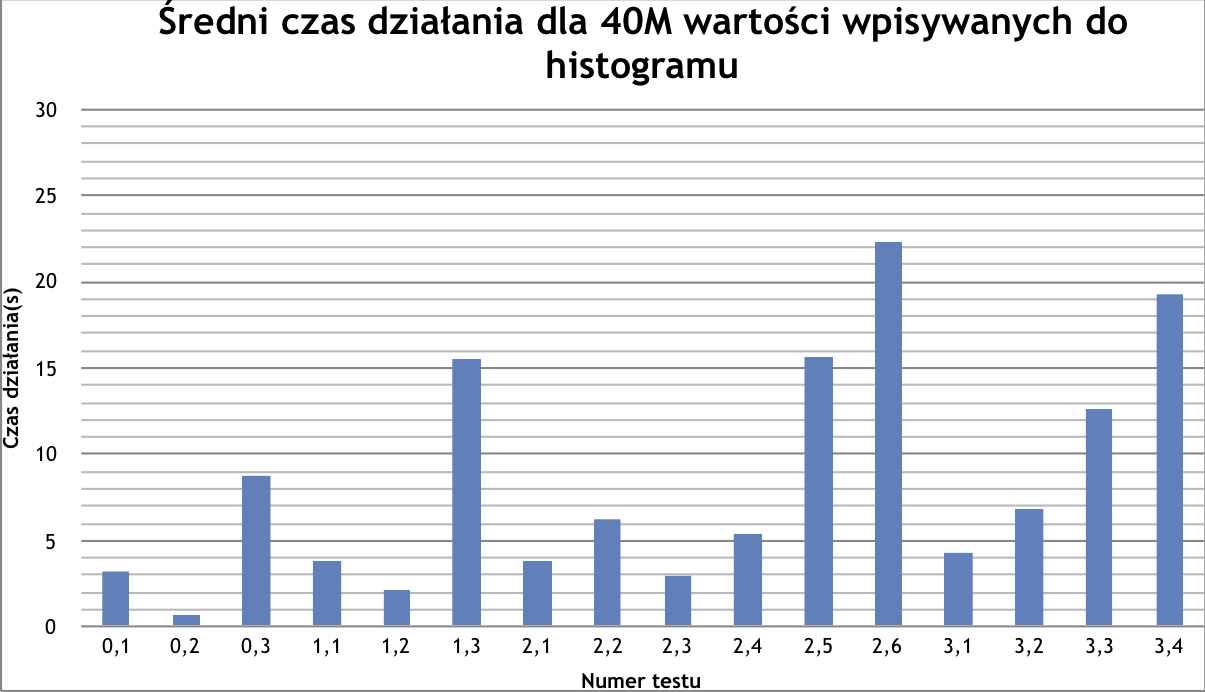
\includegraphics[width=1\textwidth]{img/avg_run_time.png}
\caption{
Wszystkie wyniki są średnią z 10 uruchomień.
0 - czas losowania 40M danych; 
1 - bezpośrednie wypełnianie histogramu z algorytmu;
2 - zmienna monitorowana bez synchronizacji wątków;
3 - zmienna monitorowana z synchronizacją wątków;
0,1 - jeden wątek;
0,2 - 800 wątków;
0,3 - 800 wątków + mutex;
1,1 - jeden wątek;
1,2 - 800 wątków, kompletność danych 5,15\%;
1,3 - 800 wątków + mutex;
2,1 - jeden wątek, histogram utworzony raz;
2,2 - jeden wątek, histogram tworzony za każdym razem;
2,3 - 800 wątków, histogram utworzony raz, kompletność danych 9,6\%;
2,4 - 800 wątków, histogram tworzony za każdym razem, kompletność danych 4,48\%;
2,5 - 800 wątków + mutex, histogram utworzony raz;
2,6 - 800 wątków + mutex, histogram tworzony za każdym razem;
3,1 - jeden wątek, histogram utworzony raz;
3,2 - jeden wątek, histogram tworzony za każdym razem;
3,3 - 800 wątków, histogram utworzony raz;
3,4 - 800 wątków, histogram tworzony za każdym razem;
}
\label{fig:athena:avgRunTime}
\end{figure}

Podczas implementacji zabezpieczeń przetwarzania wielowątkowego dla GenericMonitoringTool, bardzo ważne było sprawdzenie jak duży jest narzut na synchronizacje wątków. 
Przetestowane zostało kilka rozwiązań, w czego rezultacie najlepsze okazało się zastosowanie `mutex`'a z biblioteki standardowej C++ wewnątrz zmiennej monitorowanej. 
Rysunek~\ref{fig:athena:avgRunTime} prezentuje wyniki tych testów. 
W ich przypadku, czas działania algorytmu jest pomijalnie mały, gdyż jest w nich losowana pojedyncza wartość liczbowa.
W rzeczywistym użyciu spodziewane jest, że czas wykonywania algorytmu będzie dużo większy od czasu potrzebnego na obsługę sekcji krytycznej. 
Najbardziej reprezentatywne na tym wykresie są przypadki 1,3 oraz 3,3.

1,3 jest wynikiem działania kodu, który wykorzystuje mechanizmy dostępne przed refaktoryzacją.
Użytkownik samemu obsługuje synchronizacje z wykorzystaniem mutex'a dla 800 wątków i wypełnia histogram odwołując się bezpośrednio do obiektów frameworka ROOT.

3,3 jest wynikiem działania kodu wykorzystującego zmienną monitorowaną, która w sposób niewidoczny dla użytkownika dba o synchronizację i wypełnienie histogramów ROOT. 

Testy były przeprowadzane na wirtualizowanym środowisku LXPLUS~\cite{cern-lxplus}, które jest współdzielone między wieloma użytkownikami, co może obciążać te wyniki błędem. 
Jednak najważniejszy wniosek z nich jest taki, że GenericMonitoringTool nie wprowadza znaczącego narzutu na obsługę histogramów w porównaniu do podejścia bezpośredniego.
Różnica w czasie wykonania na korzyść zmiennej monitorowanej może być również spowodowana optymalizacjami dokonanymi przez kompilator. 

\subsection{Testy jednostkowe}
Jednym z wymogów przy tworzeniu nowego kodu do monitoringu było to, że musi on posiadać testy jednostkowe.
Aby to osiągnąć, został on zaprojektowany w sposób umożliwiający jego testowanie - wprowadzenie interfejsów i klas bazowych, oraz użycie wstrzykiwania zależności.
Pozwala to odizolować kod który chcemy zweryfikować i napisać testy które opiszą oczekiwane od niego zachowanie.

Athena dostarcza podstawowe narzędzia do tworzenia testów jednostkowych, takie jak np. asercje, jednak nie definiuje ona ich struktury.
Aby to usystematyzować powstał szablon pliku z testami dla kodu monitoringu, przedstawiony został na listingu~\ref{lst:athena:unit_test_template}.

\lstinputlisting[
	style=cpp, 
	caption=Szablon pliku z testami jednostkowymi, 
	label={lst:athena:unit_test_template}
]{ExampleClassTestSuite.cxx}

Szablon podzielony jest na następujące sekcje:
\begin{itemize}
\item Zarejestrowane testy - w tej części, użytkownik jest zobowiązany do zadeklarowania testów, które mają zostać uruchomione. Wykorzystane jest tutaj makro `REGISTER\_TEST\_CASE`, którego celem jest uproszczenie tego procesu. Jej istnienie wynika z ograniczeń języka C++, który nie pozwala pobrać listy wszystkich dostępnych metod dla danej klasy.
\item Kod testów - definiuje ona metody `beforeEach` - wywoływana przed każdym testem - i `afterEach` - wywoływana po każdym teście. W razie potrzeby, użytkownik powinien w nich odpowiednio przygotować środowisko do testów. W tej sekcji użytkownik definiuje metody, które posłużą do weryfikacji poprawności zachowania testowanej klasy. Ich nazwa powinna zaczynać się od `test\_should`.
\item Metody pomocnicze - miejsce na metody pomocnicze zdefiniowane przez użytkownika na potrzeby testów.
\item Inicjalizacja i uruchomienie - w tej sekcji zdefiniowany jest sposób uruchomienia testów.
\item Rejestracja testów - tej części metody testowe są przygotowywane do uruchomienia. Użytkownik nie powinien jej modyfikować.  
\item Pola klasy - zawiera deklaracje wszystkich zmiennych. `m\_testObj` jest specjalną zmienną, która zawiera obiekt testowanej klasy.  
\end{itemize}

Szablon ten został wykorzystany na potrzeby przetestowania wszystkich najważniejszych komponentów GenericMonitoringTool.

\begin{cpp}[caption=Jeden z testów zdefiniowanych w ramach HistogramFactoryTestSuite~\cite{histogram-factory-test-suite}, label={lst:athena:histogram_factory_test_suite}]
void test_shouldRegisterAndReturnTH1DHistogram() {
   TH1D* const histogram = createHistogram<TH1D>("TH1D");
   VALUE(m_histSvc->exists("/HistogramFactoryTestSuite/TH1D")) EXPECTED(true);
   VALUE(histogram) NOT_EXPECTED(nullptr);
}
\end{cpp}

W celu poprawnego odizolowania testowanego kodu, powstały klasy dostępne tylko na potrzeby testów - `mocki`, których zadaniem jest imitowanie prawdziwych komponentów GenericMonitoringTool.
Ich zachowanie jest całkowicie pod kontrolą użytkownika.
Takie obiekty, w połączeniu ze wstrzykiwaniem zależności, umożliwiają całkowite uniezależnienie weryfikowanego kodu od innych komponentów.

% !TEX root = main.tex
\section{Możliwe ścieżki rozwoju narzędzia GenericMonitoringTool}
\begin{itemize}
\item usunięcie mutex'ów
\item aktualizacja frameworka ROOT do wersji zawierającej wewnętrzną synchronizację wątków
\item dodawanie nowych funkcjonalności w ramach potrzeb
\end{itemize}

//TODO
% !TEX root = main.tex
\section{Podsumowanie}
podsumowanie
% !TEX root = main.tex
\newpage
\section{Bibliografia}
\printbibliography[heading=none]

\end{document}